\documentclass{beamer}

\usepackage{beamerthemesplit}
\usepackage{amsmath}
\usepackage{amsfonts}
\usepackage{amssymb}
\usepackage{cancel}
\usepackage{tkz-graph}

\makeatletter
\newcommand{\reallytiny}{\@setfontsize{\srcsize}{2pt}{2pt}}
\makeatother

\mode<presentation>
{
  \usetheme{AnnArbor}
  % or ...

  %\setbeamercovered{transparent}
  % or whatever (possibly just delete it)
}

\usepackage[english]{babel}
% or whatever

\usepackage[latin1]{inputenc}
% or whatever

\usepackage{times}
\usepackage[T1]{fontenc}

\title{From Tracker to PianoRoll and Back}

\author{Nil Geisweiller}

\date[Sonoj-19]
{Sonoj 2019, Cologne, Germany}

\begin{document}

\begin{frame}
  \maketitle
\end{frame}

\begin{frame}
  \begin{center}
    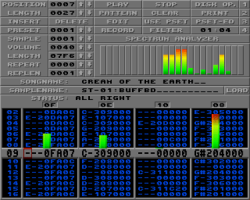
\includegraphics[scale=1.0]{images/protracker.png}
  \end{center}
\end{frame}

\begin{frame}
  \begin{center}
    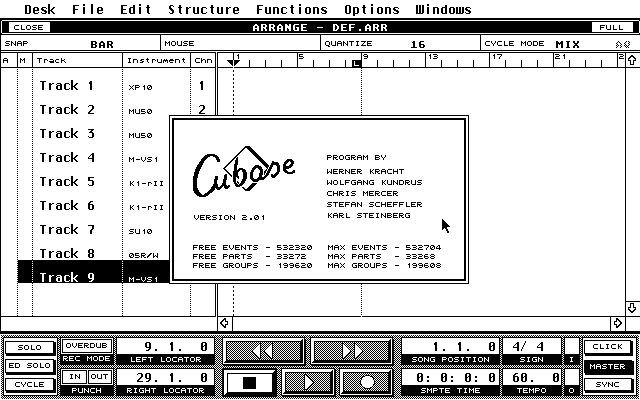
\includegraphics[scale=0.5]{images/cubase_2-01_atari_st.png}
  \end{center}
\end{frame}

\begin{frame}
  \begin{center}
    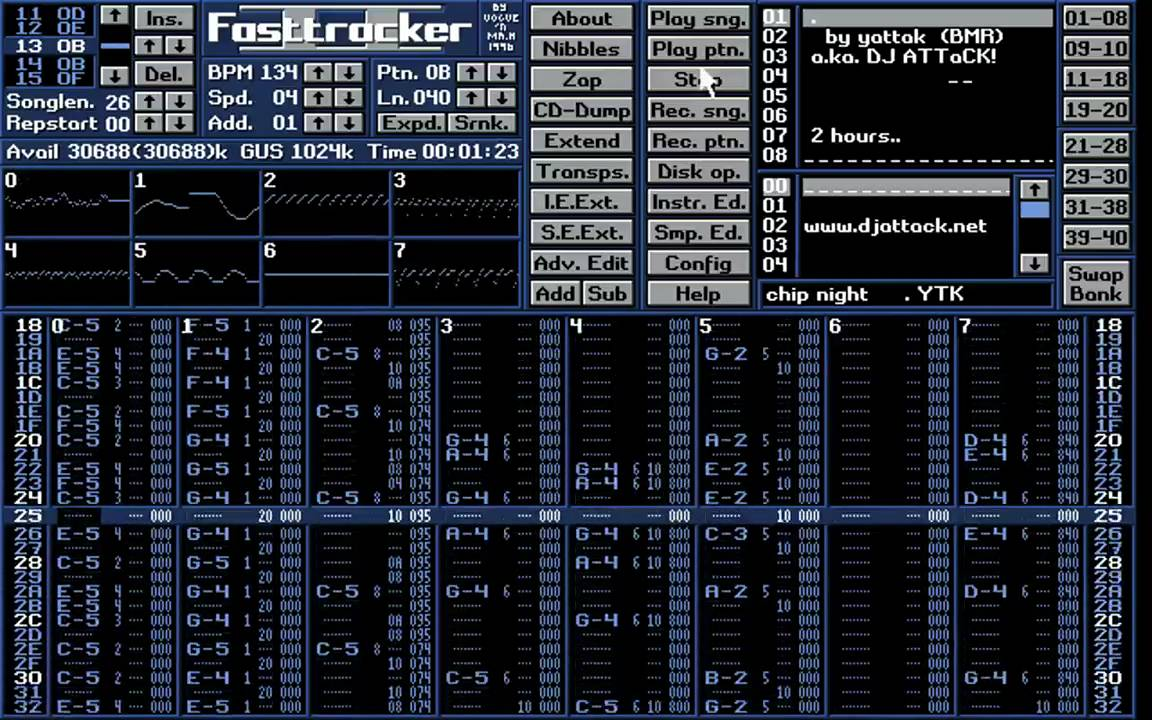
\includegraphics[scale=0.3]{images/fasttracker2.jpg}
  \end{center}
\end{frame}

\begin{frame}
  \begin{center}
    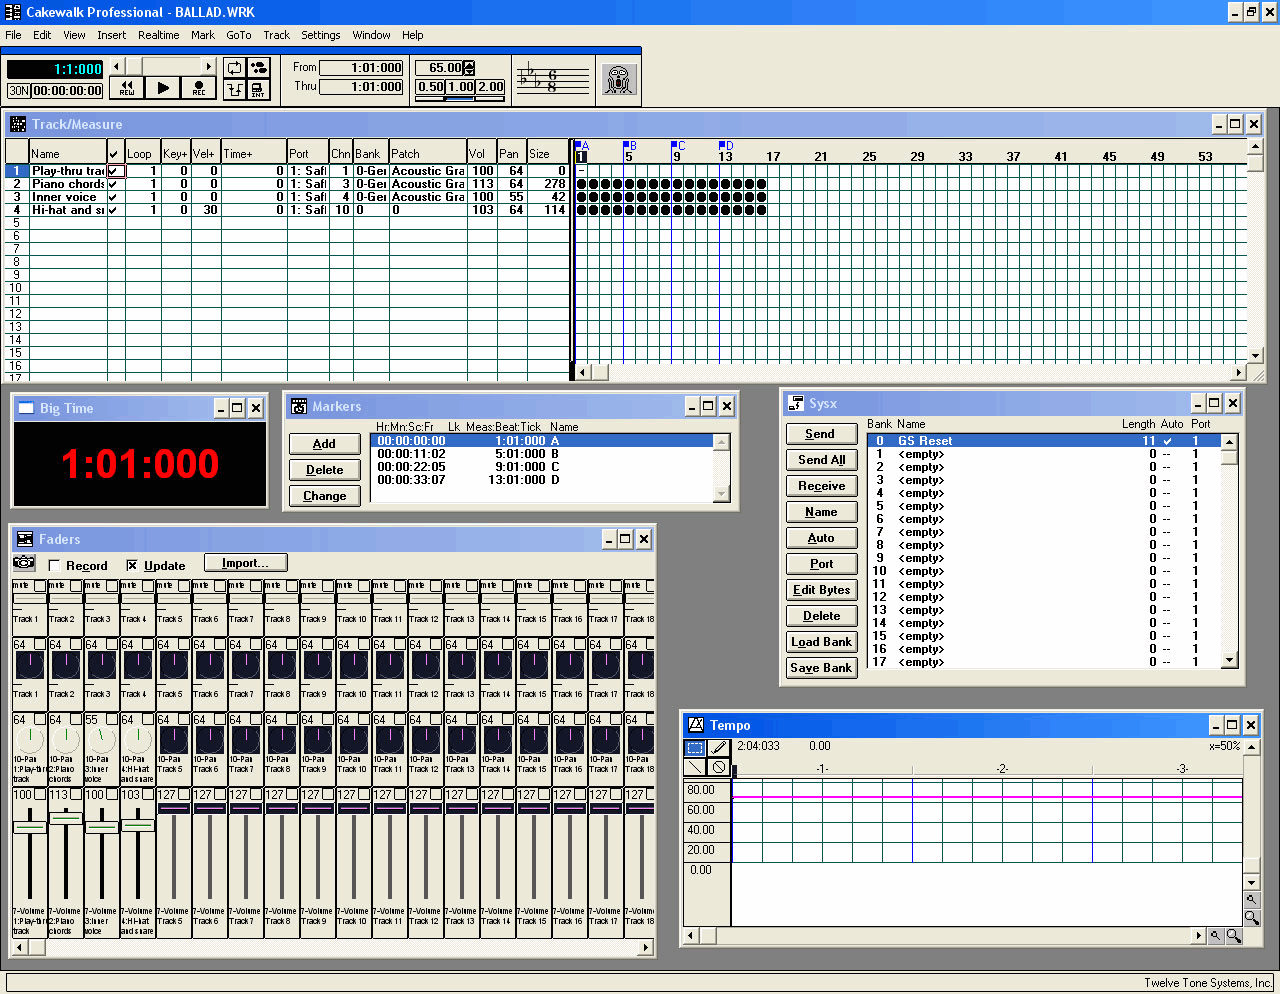
\includegraphics[scale=0.25]{images/cakewalk.png}
  \end{center}
\end{frame}

\begin{frame}
  \begin{center}
    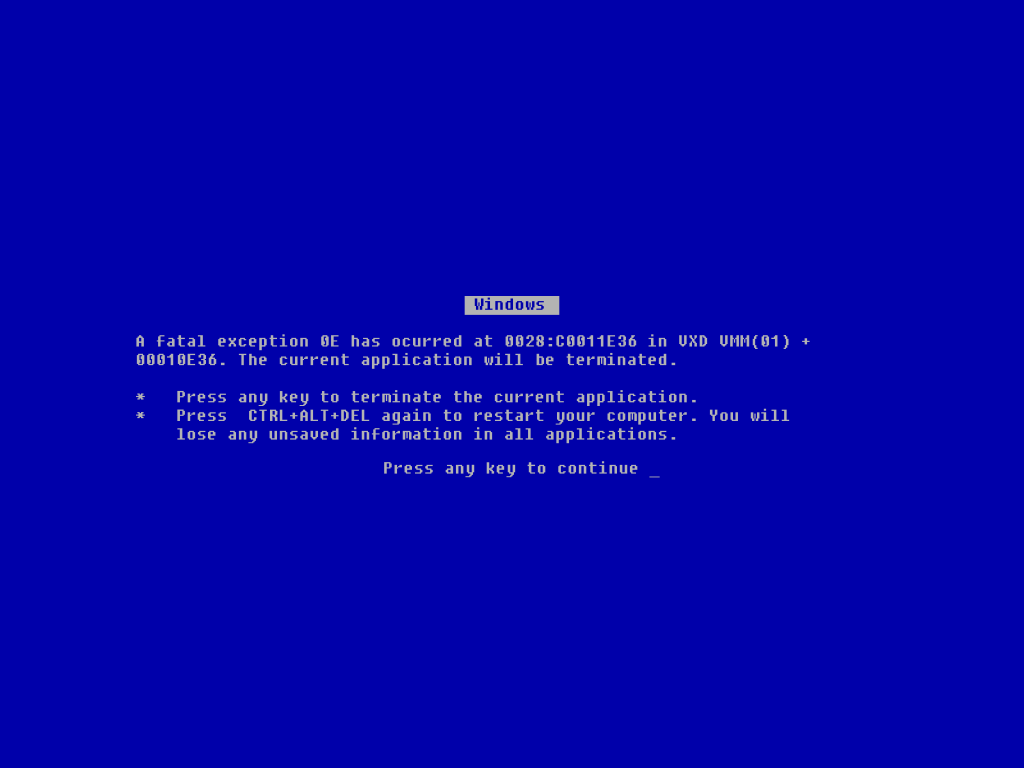
\includegraphics[scale=0.30]{images/Windows_9x_Blue_Screen_of_Death_recreated_in_Fixedsys.png}
  \end{center}
\end{frame}

\begin{frame}
  \begin{center}
    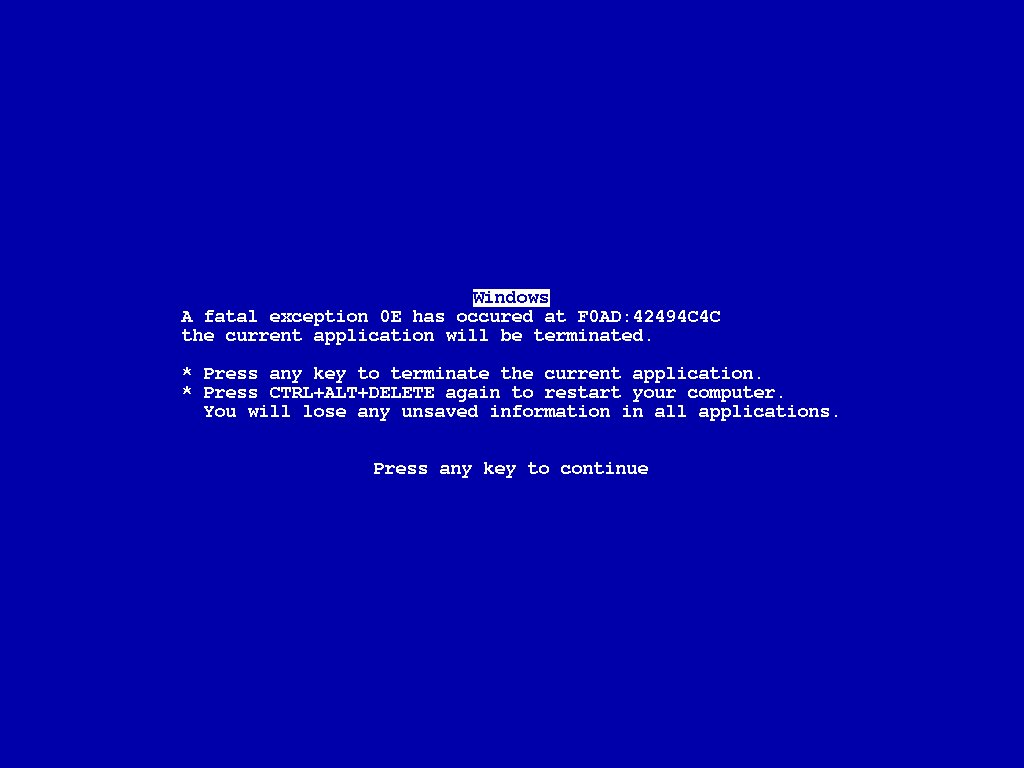
\includegraphics[scale=0.30]{images/fix-bsod-win7.jpg}
  \end{center}
\end{frame}

%% \begin{frame}
%%   \begin{center}
%%     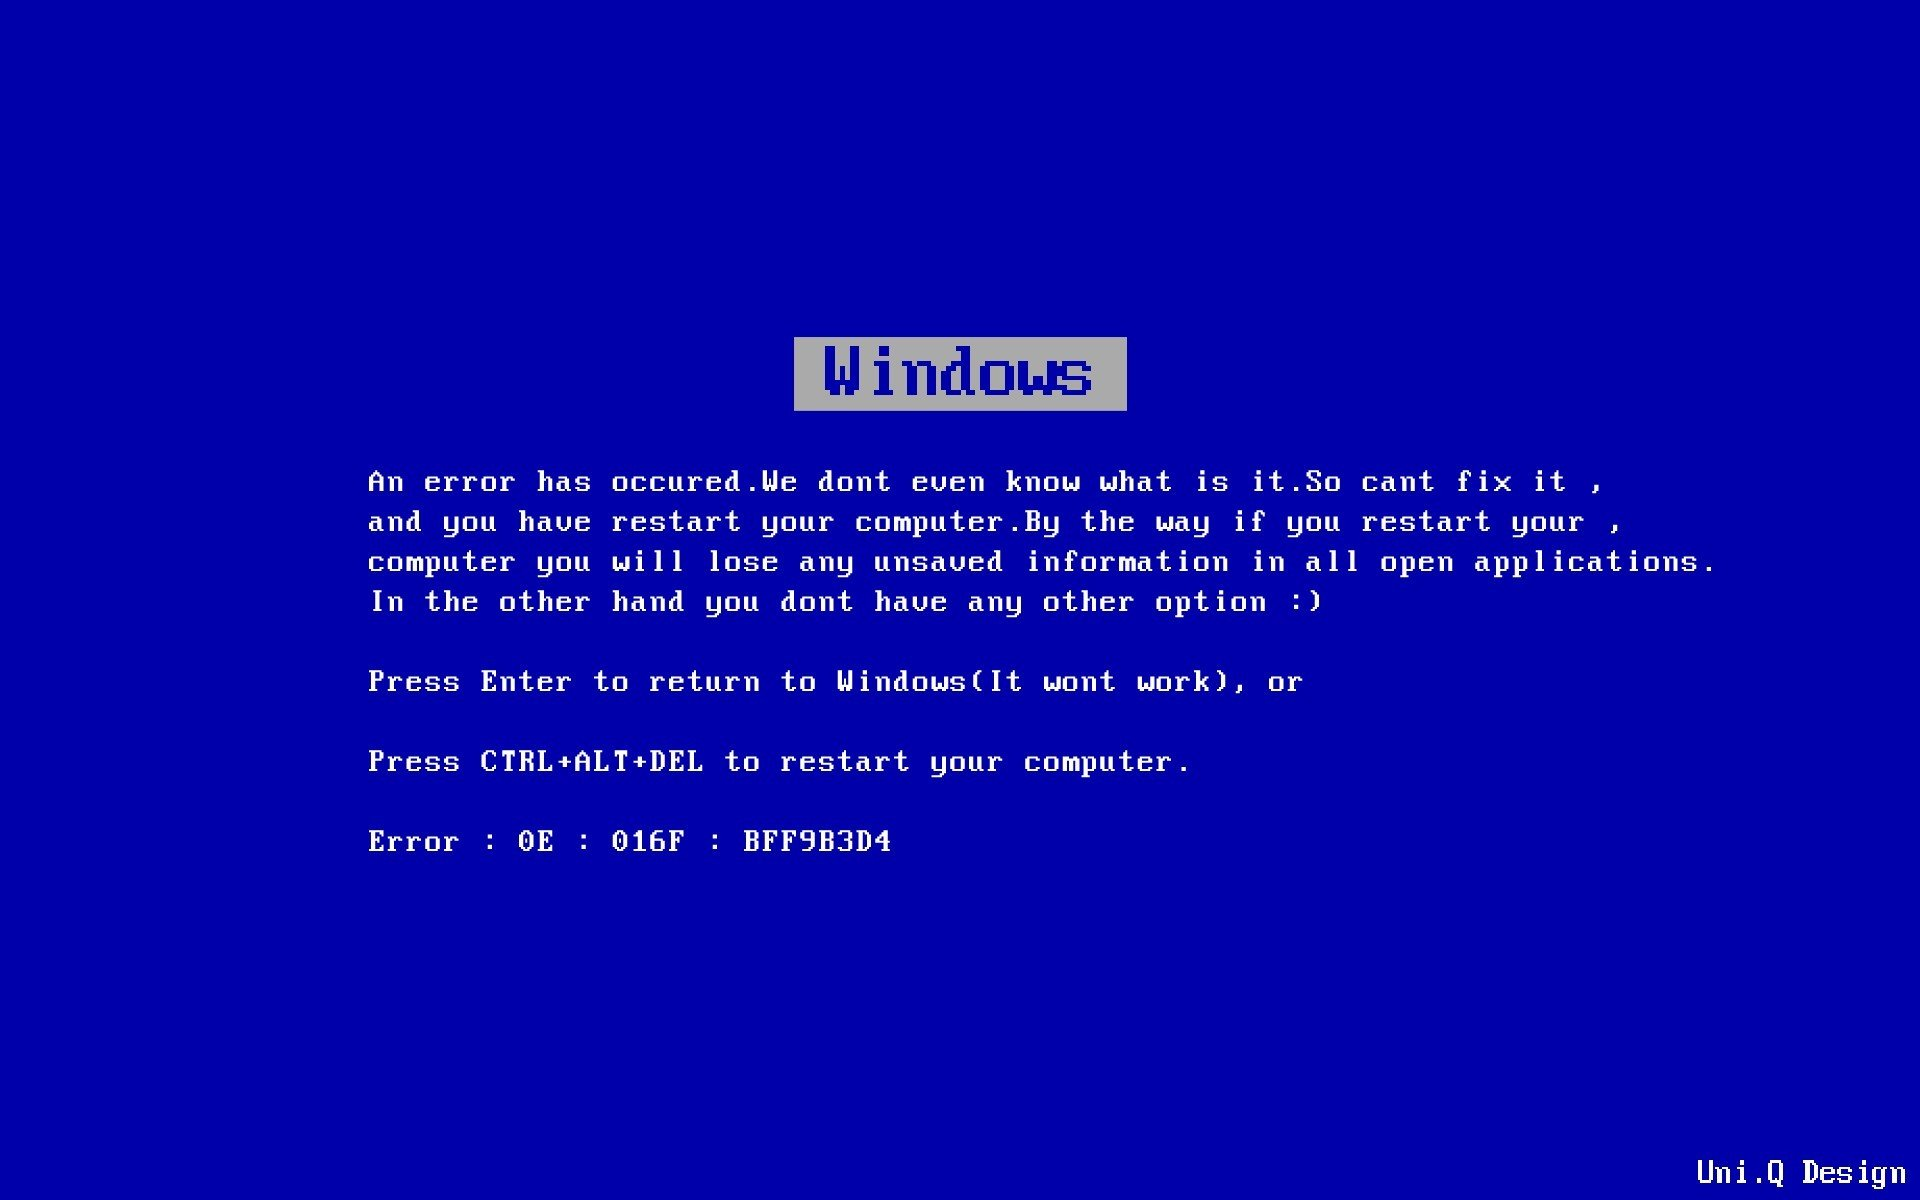
\includegraphics[scale=0.16]{images/53776-Microsoft_Windows-Blue_Screen_of_Death.jpg}
%%   \end{center}
%% \end{frame}

\begin{frame}
  \begin{center}
    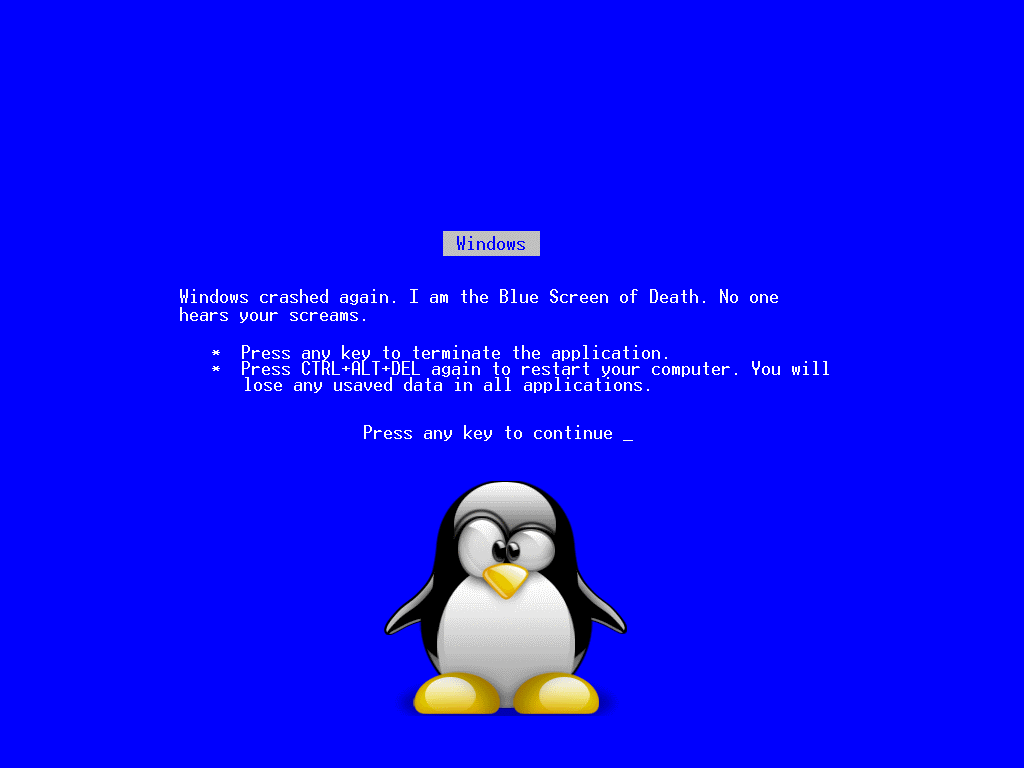
\includegraphics[scale=1.2]{images/hb7nfO.png}
  \end{center}
\end{frame}

\begin{frame}
  \begin{center}
    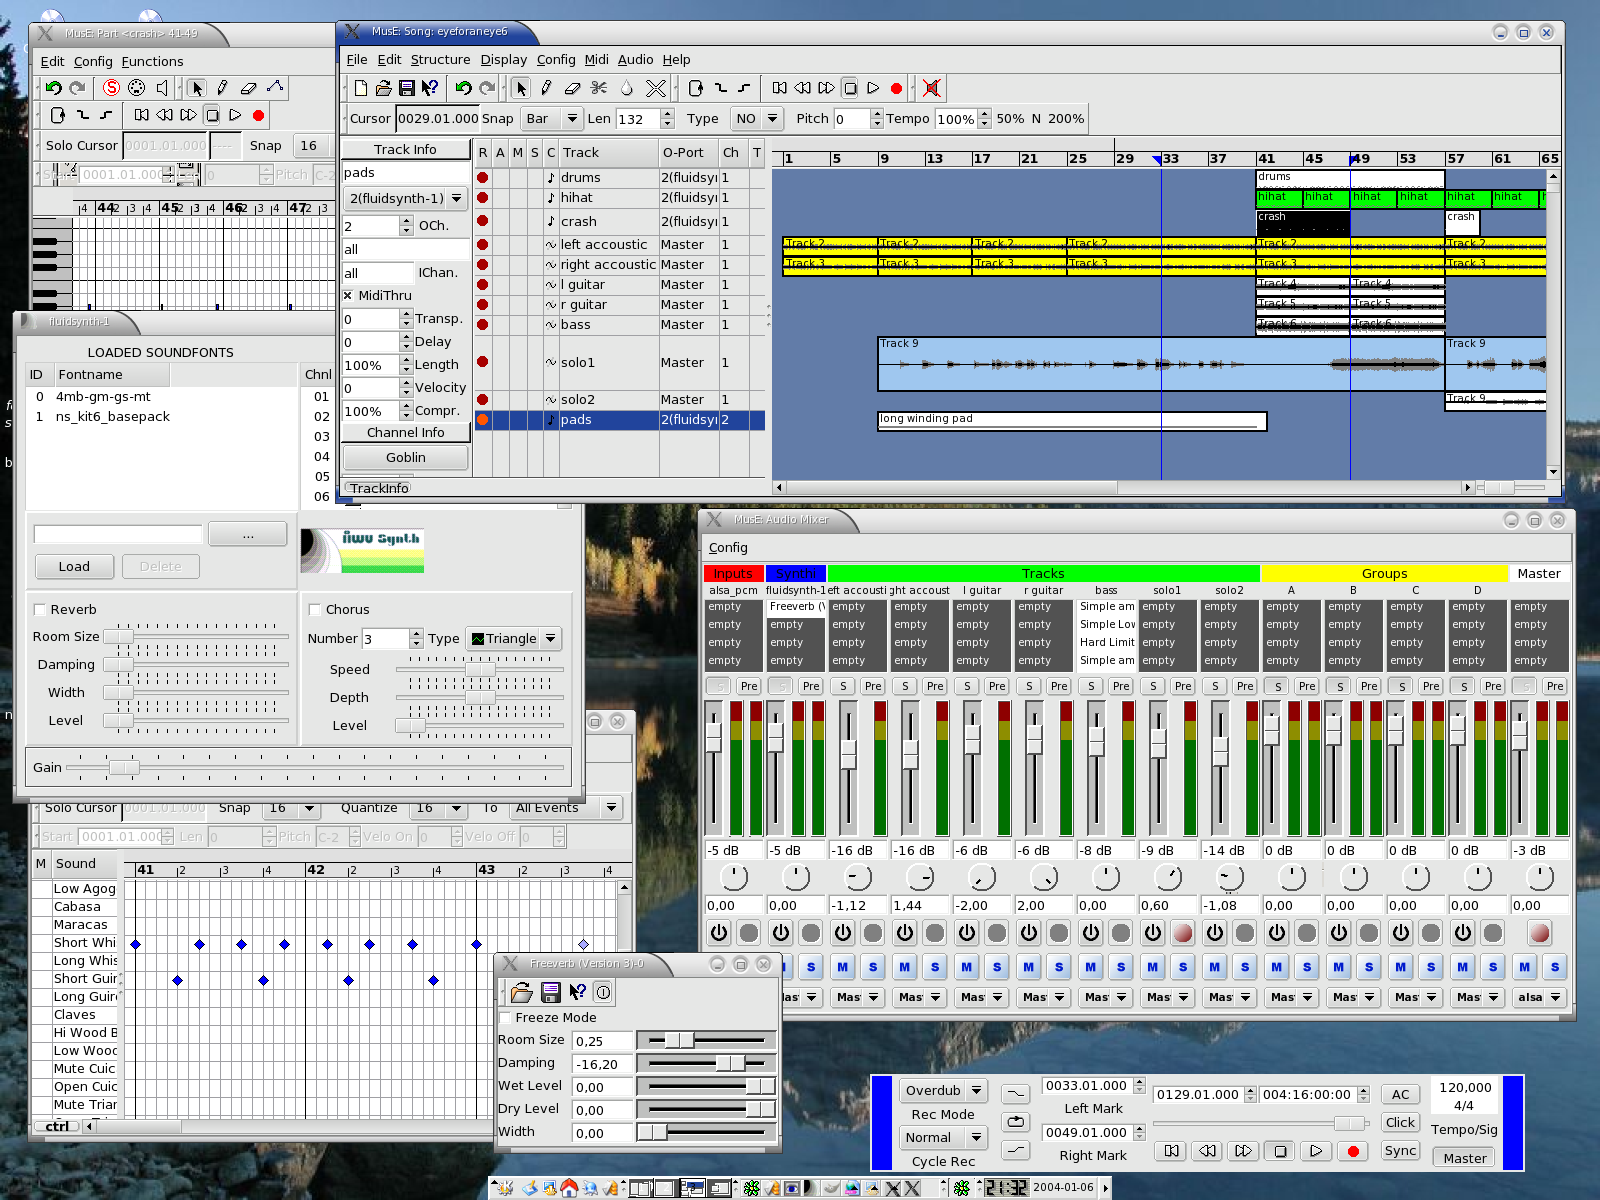
\includegraphics[scale=0.2]{images/muse_desktop.png}
  \end{center}
\end{frame}

\begin{frame}
  \begin{center}
    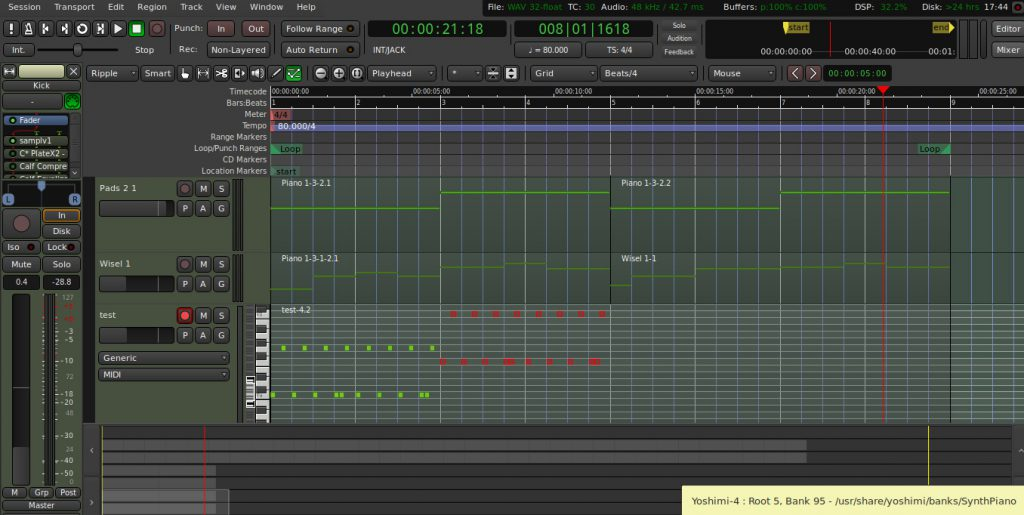
\includegraphics[scale=0.33]{images/Screenshot-from-2017-08-01-17-44-03-1024x515.jpg}
  \end{center}
\end{frame}

\end{document}
